\documentclass[border=10pt]{standalone}
\usepackage{pgfplots}
\begin{document}
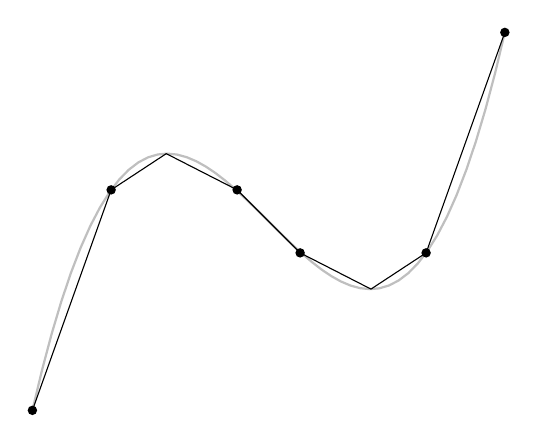
\begin{tikzpicture}
  \draw[domain=-3:3,samples=50,color=gray!50,thick] plot (\x, \x^3/5 - \x);
  \foreach \x/\y in { -3/-2.4, -2/0.4, -0.4/0.4,
    0.4/-0.4, 2/-0.4, 3/2.4 }
      \fill (\x,\y) circle (0.6mm);
  \draw plot coordinates {
    (-3,-2.4) (-2,0.4) (-1.3,0.86) (-0.4,0.4)
    (0.4,-0.4) (1.3,-0.86) (2,-0.4) (3,2.4) };
\end{tikzpicture}
\end{document}
